\documentclass[a4paper]{article}
\usepackage[12pt]{extsizes}
\usepackage{fullpage}
\usepackage{cmap}
\usepackage{graphicx}
\usepackage{multirow}
\usepackage{amsmath,amsthm,amsfonts,amssymb,amscd}
\usepackage{mathrsfs}
\usepackage{listings}
\usepackage[utf8]{inputenc}
\usepackage[T1]{fontenc}
\usepackage[english, russian]{babel}


\usepackage{fancyhdr} % для колонтитулов
\pagestyle{fancy}
\fancyhf{}
\setlength{\headheight}{0pt}
\renewcommand{\headrulewidth}{0pt}

\newcommand{\anonsection}[1]{ \section*{#1} \addcontentsline{toc}{section}{\numberline {}#1}}

\lstset{
	language=Python,
	extendedchars=\true,
	inputencoding=utf8x,
	commentstyle=\itshape,
	stringstyle=\bf,
	belowcaptionskip=5pt }

\begin{document}
	\begin{center}
		\textbf{
			МИНИСТЕРСТВО ОБРАЗОВАНИЯ РЕСПУБЛИКИ БЕЛАРУСЬ \\
			БЕЛОРУССКИЙ ГОСУДАРСТВЕННЫЙ УНИВЕРСИТЕТ \\
			Факультет прикладной математики и информатики
		} \\
		
		\vspace{1em}
		
		\text {
			Кафедра математического моделирования и анализа данных
		}
	\end{center}
	
		\vspace{10em}
		
	\begin{center}
		\textbf{
			ЦУРАНОВ НИКИТА ВАСИЛЬЕВИЧ \\
			\vspace{1em}
			СТАТИСТИЧЕСКИЙ АНАЛИЗ ВРЕМЕННЫХ РЯДОВ \\
			С ПОМОЩЬЮ ВЕЙВЛЕТ ПРЕОБРАЗОВАНИЙ
		}
		
		\vspace{3em}
		Курсовая работа \\
		Студента 3 курса 7 группы
		
	\end{center}
	
	\vspace{10em}
	
	\begin{minipage}{0.4\textwidth}
		\begin{center}
			Допустить к защите \\
			\textbf{Руководитель работы} \\
			\underline{
				\qquad\qquad\qquad
				\qquad\qquad\quad
			} \\
			«\qquad»\underline{\qquad\qquad\qquad} 2020
		\end{center}
	\end{minipage}
	\hfill
	\begin{minipage}{0.4\textwidth}
		\begin{center}
			\textbf{Руководитель} \\
			\textit{Лобач Виктор Иванович} \\ 
			доцент кафедры ММАД \\ 
			канд. физ.-мат. наук
		\end{center}
	\end{minipage}
	
	\fancyfoot[C]{\large{Минск, 2020}}

	\newpage
	
	\fancyfoot[C]{\thepage}
	
	
	\tableofcontents
	\newpage
	
	
	\anonsection{Введение}
	
	Вейвлет-преобразование представляет собой синтез идей, которые возникли за многие годы из разных областей, таких как математика и обработка сигналов. Вообще говоря, вейвлет-преобразование --- это инструмент, который делит данные, функции или операторы на разные частотные компоненты, а затем изучает каждый компонент с разрешением, соответствующим его масштабу$^{[1]}$.
	
	Таким образом, вейвлет-преобразование используется для обеспечения экономного и информативного математическое представление многих объектов, представляющих интерес$^{[2]}$. В настоящее время многие компьютерные программные пакеты содержат быстрые и эффективные алгоритмы для преобразования вейвлетов. Благодаря такой легкой доступности вейвлеты быстро завоевали популярность среди ученых и инженеров, как в области теоретических исследований, так и в области применения. Прежде всего, вейвлеты широко применяются в таких областях компьютерных наук, как обработка изображений, компьютерное зрение, управление сетями и анализ данных. За последнее десятилетие интеллектуальный анализ данных или базы данных обнаружения знаний стали важной областью как в академия и в промышленности. Интеллектуальный анализ данных - это процесс автоматического извлечения новых полезных и понятных шаблонов из большой коллекции данных.
	
	Теория вейвлетов, естественно, может сыграть важную роль в анализе данных, поскольку она хорошо обоснована и имеет очень практическое применение. У вейвлетов есть много благоприятных свойств, таких как исчезающие моменты, иерархическая структура с разложением по иерархии и многоразрешению, линейная временная и пространственная сложность преобразований, декоррелированные коэффициенты и широкий спектр базовых функций. Эти свойства могут обеспечить значительно более эффективные и эффективные решения многих проблем анализа данных. Во-первых, вейвлеты могут обеспечивать представление данных, которые делают процесс сбора данных более эффективным и точным. Во-вторых, вейвлеты могут быть включены в ядро многих алгоритмов сбора данных.
	
	Хотя стандартные вейвлет-приложения в основном используются для данных, которые имеют временную / пространственную локализацию (например, временные ряды, данные потоков и данные изображений), вейвлеты также успешно применяются в различных областях при извлечении данных. На практике широкое разнообразие методов, связанных с вейвлетами, было применено для решения целого ряда проблем интеллектуального анализа данных.
	
	В этой работе представляются необходимые математические основы для понимания и использования вейвлетов, а также краткий обзор исследований вейвлет-приложений
	
	\newpage
	
	\section{Вейвлеты Хаара и их свойства}
	Рассмотрим основные характеристики вейвлетов Хаара.
	
	Материнская функция$^{[3]}$ задается следующим образом: 
	$$
		\psi(x) = 
		\begin{cases}
			 1, & x \in [0, 0.5) \\
			-1, & x \in [0.5, 1) \\
			 0, & \text{иначе}
		\end{cases}
	$$
		
	Масштабирующая функция определяется как:
	$$
		\phi(x) =
		\begin{cases}
			1, & x \in [0, 1) \\
			0, & \text{иначе}
		\end{cases}
	$$
	
	Система базисных вейвлетов получается путем растяжения и смещения материнского вейвлета:
	$$ 
		\psi_{a, b}(x) = 2^{\frac{a}{2}}\psi(2^at-b);
		a \in N_0, b = 0...2^a-1
	$$
	
	Свойства вейвлетов$^{[4]}$:
	
	\begin{itemize}
		\item $\psi(x)$ абсолютно интегрируемая и принадлежит $L^2$:
		$$
			\int_{-\infty}^{\infty} |\psi(x)|dx < \infty 
			\text{ и }
			\int_{-\infty}^{\infty} |\psi(x)|^2dx < \infty 
		$$
		\item Среднее равно нулю, а норма равна единице:
		$$
			\langle f, g \rangle = \int_{-\infty}^{\infty} f(x)g(x)dx
			\text{ --- скалярное произведение в }L^2
		$$ 
		$$
			\int_{-\infty}^{\infty} \psi(x)dx = 0 
			\text{ и }
			\int_{-\infty}^{\infty} \psi(x)^2dx = 1
		$$
		\item Вейвлеты Хаара так же является ортонормированными:
		$$
			\langle
				\psi_{a, b}(x),
				\psi_{i, j}(x)
			\rangle = 
			\begin{cases}
				1, & a, b = i, j \\
				0, & \text{иначе} 
			\end{cases}
		$$
	\end{itemize}
	
	\newpage
	
	\section{Преобразование Фурье и вейвлет-преобразование}
	
	Преобразование Фурье[5] функции вещественной переменной задается формулой:
	$$ \hat{f}(w) = \frac{1}{\sqrt{2\pi}} \int_{-\infty}^{\infty} f(x) e^{-ixw} dx $$
	Формула обращения:
	$$ f(x) = \frac{1}{\sqrt{2\pi}} \int_{-\infty}^{\infty} \hat{f}(w) e^{ixw} dw $$
	
	В контексте анализа временных рядов, которые можно рассматривать как сигналы, преобразование Фурье позволяет перевести сигнал из временного представления в частотное.
	
	Но у преобразования Фурье есть недостаток. Т.к. мы получаем только частотный спектр, то результат преобразования для суммы двух синусоид и синусоиды, переходящей в другую, (с теми же частотами и на таком же временном промежутке) будет неотличим (преобразование Фурье используется только для периодичных функций).
	
	Если нам нужно больше, чем просто анализ спектра частот, то существует оконное преобразование Фурье, а также вейвлет-анализ.
	
	\begin{center}
		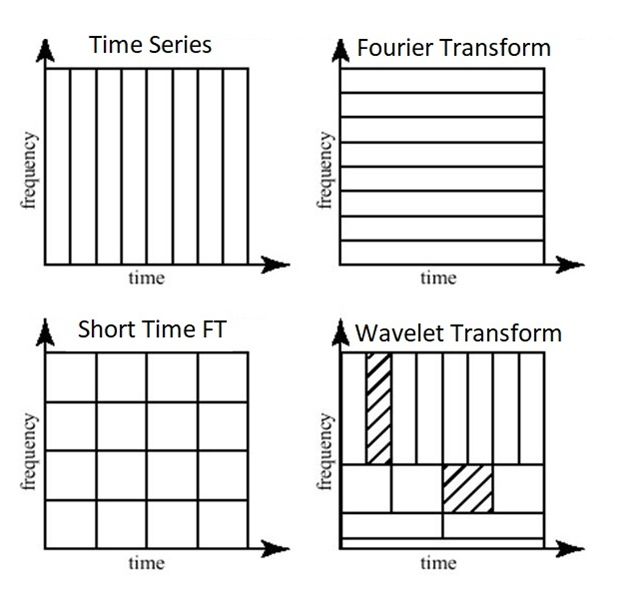
\includegraphics[scale=0.4]{./img1.jpg}
	\end{center}
	 
	Вейвлет-преобразование $ W(a,b) = \int_{-\infty}^{\infty} f(x) \psi_{a, b}(x)dx $ отличается от преобразования Фурье выбором анализирующей функции. Но для разложения в ряд Фурье мы накладывали условие ортогональности, и благодаря этому мы раскладывали функцию по заданному базису. С вейвлетами, в общем случае, мы так сделать не можем, но мы можем посмотреть насколько заданная функция похожа на наш вейвлет в заданный момент времени. Момент времени задается через растяжение и смещение анализирующей функции, а схожесть определяется величиной коэффициента.
	
	Вейвлет Хаара обладает ортогональностью, а значит мы можем провести разложение по вейвлет-базису. С этим мы подходим к задаче анализа.
	
	\newpage
	
	\section{Задачи анализа и синтеза}
	
	\subsection{Задача анализа}
	
	Задана анализа состоит в получении коэффициентов разложения. Для работы будем использовать вейвлеты Хаара. Формулы для непрерывного преобразования:
	
	$$ 
		c_{a, b} = \int_{-\infty}^{\infty}
		 x(t)\psi_{a, b}(t) dt
		\text{; }
		s = \int_{-\infty}^{\infty} x(t)\phi(t) dt$$
	$$ 
		a \in N_0, b = 0...2^a-1, a=0...M
		\text{, где M --- количество уровней разложения} 
	$$
	
	Данные формулы работают для разложения функции на промежутке [0, 1). Для разложения на ином промежутке можно расширить базис:
	
	\begin{itemize}
		\item  Введение в базис дополнительных членов (полученных большим смещением). Таким образом можем получить промежуток $[0, n)$, где $n \in N$
		
		\item Сдвиг материнского вейвлета $\psi'(t) = \psi(t - C)$ даст промежуток $[C, C + 1)$
		
		\item Растяжение материнского вейвлета $\psi'(t) = \psi(tC)$ дает промежуток $[0, C)$
	\end{itemize}

	\begin{minipage}{0.45\textwidth}
		\begin{center}
			Восстановление непрерывной функции на отрезке [0, 1] \\ с 4 уровнями
			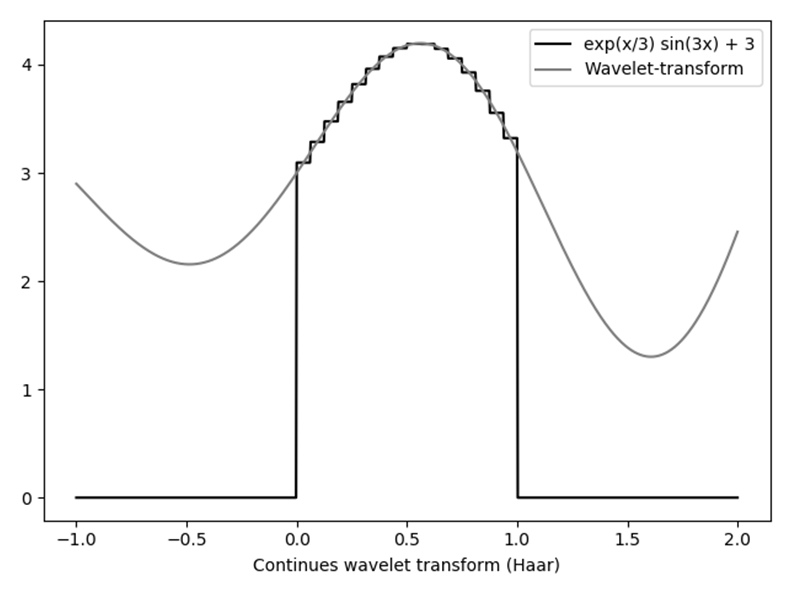
\includegraphics[scale=0.25]{./img2_1.jpg}
			Восстановление функции на отрезке [0.5, 1.5] через смещение материнского вейвлета и масштабирующей функции
			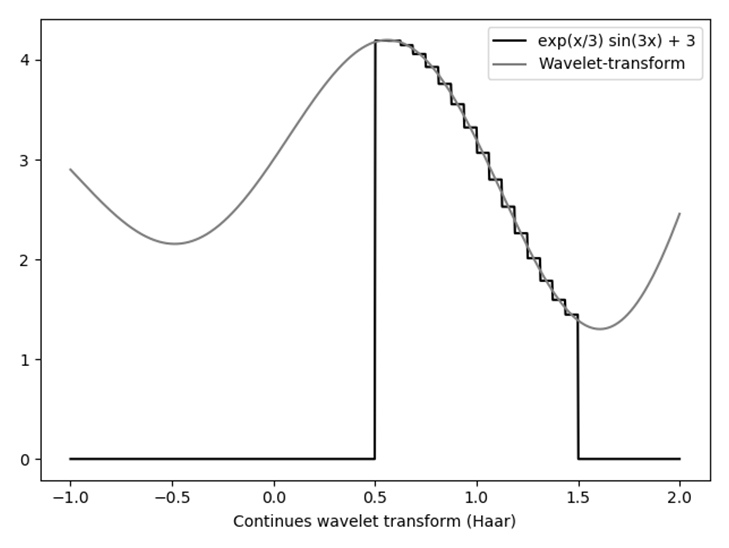
\includegraphics[scale=0.25]{./img2_3.jpg}
		\end{center}
	\end{minipage}
	\hfill
	\begin{minipage}{0.45\textwidth}
		\begin{center}
			Восстановление функции на \\ отрезке [0, 2] полученное расширением базиса
			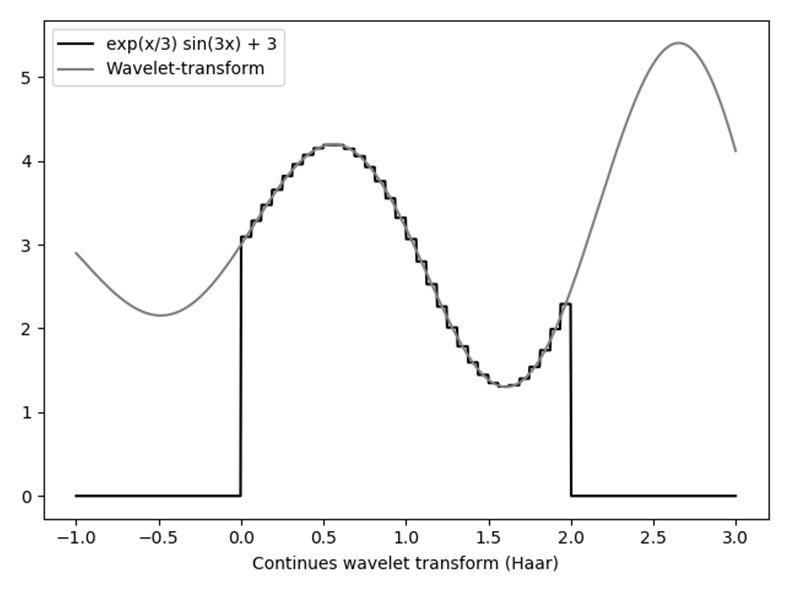
\includegraphics[scale=0.25]{./img2_2.jpg}
			Восстановление функции на отрезке [0, 1.5] через растяжение материнского вейвлета и масштабирующей функции
			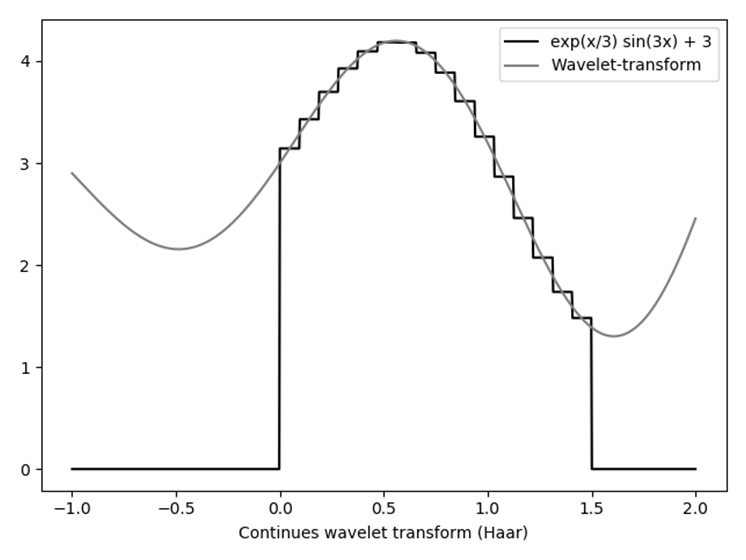
\includegraphics[scale=0.25]{./img2_4.jpg}
		\end{center}
	\end{minipage}
	
	\newpage
	
	А сам базис Хаара на отрезке [0, 1] выглядит так:
	
	\begin{center}
		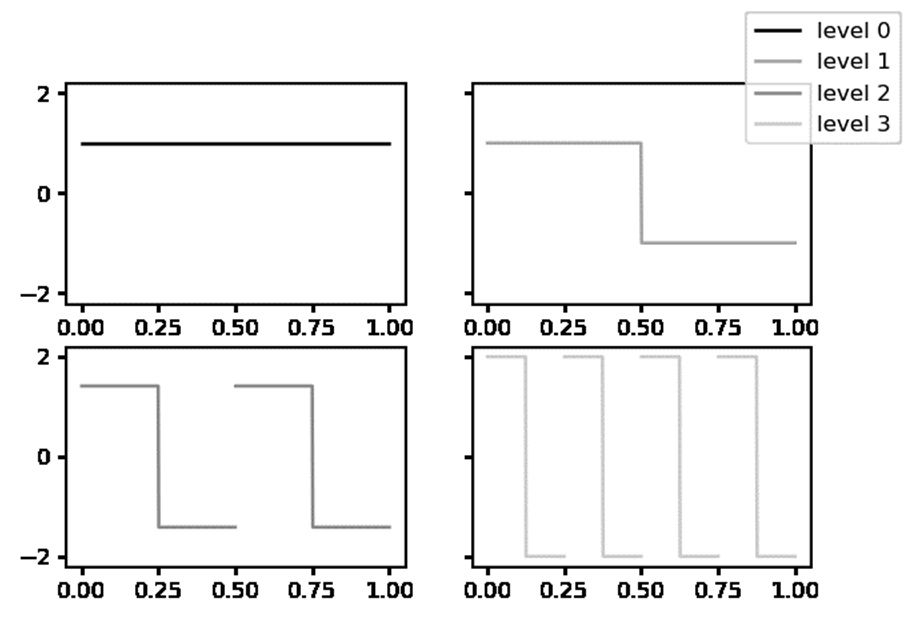
\includegraphics[scale=0.3]{./img3.jpg}
	\end{center}
	
	Но на практике мы обычно имеем дело с дискретными сигналами. Рассмотрим дискретное вейвлет-преобразование.
	
	Обычно размер данных о сигнале равен степени двойки для упрощения вычислений, тогда пусть сигнал задается как значения $X_n = x_0, ..., x_n$, где $n=2^k-1$. Рассмотрим $x_i$:
	$$ x_i = \frac{1}{2}x_i + \frac{1}{2}x_i - \frac{1}{2}x_{i-1} + \frac{1}{2}x_{i-1} =
	\frac{x_{i} + x_{i-1}}{2} + \frac{x_{i} - x_{i-1}}{2}$$
	
	Где $\frac{x_{i} + x_{i-1}}{2}$ --- аппроксимация сигнала, а $\frac{x_{i} - x_{i-1}}{2}$ --- а детализация.
	
	Такое разложение сигнала можно использовать рекуррентно:
	$$
		X = A^0,
		A^{k + 1} = 
		\begin{bmatrix}
			\frac{A^k_{2i} + A^k_{2i + 1}}{2}
		\end{bmatrix},
		D^{k + 1} = 
		\begin{bmatrix}
		\frac{A^k_{2i} - A^k_{2i + 1}}{2}
		\end{bmatrix};
		i < n_{k+1}, n_{k+1} = \frac{n_k}{2}
	$$
	
	\begin{center}
		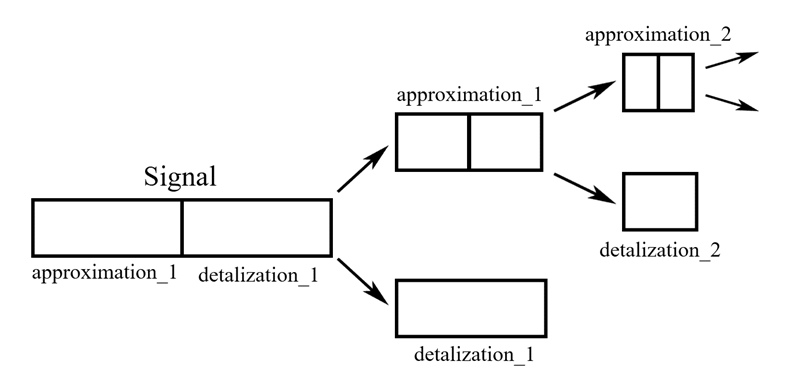
\includegraphics[scale=0.4]{./img4.jpg}
	\end{center}
	
	Этот метод позволяет получить разложение без потери точности и без вычисления самих вейвлетов, а за счет рекурсии работает асимптотически за $O(n \log(n))$. Также позволяет упростить сам сигнал, оставляя просто аппроксимацию.
	
	\subsection{Задача синтеза}
	
	Задача синтеза состоит в восстановлении сигнала по полученным коэффициентам.
	
	По тем формулам для вейвлета Хаара, что мы определили в 3.1 получаем:
	
	\begin{itemize}
		\item Для непрерывного: $ x(t) = s \phi(t) + \sum_{a=0}^{M} \sum_{b=0}^{2^a} c_{a, b} \phi_{a, b}(t) $ --- по аналогии с рядами Фурье
		\item Для дискретного: $
			A^{k - 1} = 
			\begin{bmatrix}
				A^k_i + D^k_i, A^k_i - D^k_i
			\end{bmatrix}, i < n_k
		$
	\end{itemize}

	\begin{center}
		Рассмотрим восстановление сигналов различных уровней:
		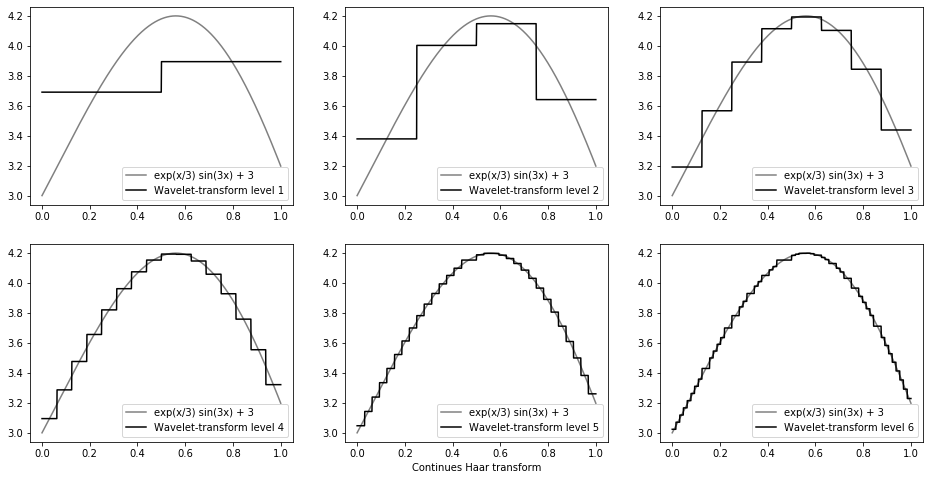
\includegraphics[scale=0.5]{./output_5_0.png}
	\end{center}
	
	\newpage
	
	\section{Компьютерные эксперименты}
	
	\subsection{Преимущество временных рядов перед преобразованием Фурье}
	
	Преобразование Фурье можно использовать либо только для периодических сигналов, либо для определения частот.
	
	Рассмотрим 2 примера:
	\begin{center}
		Сумма двух синусоид:
		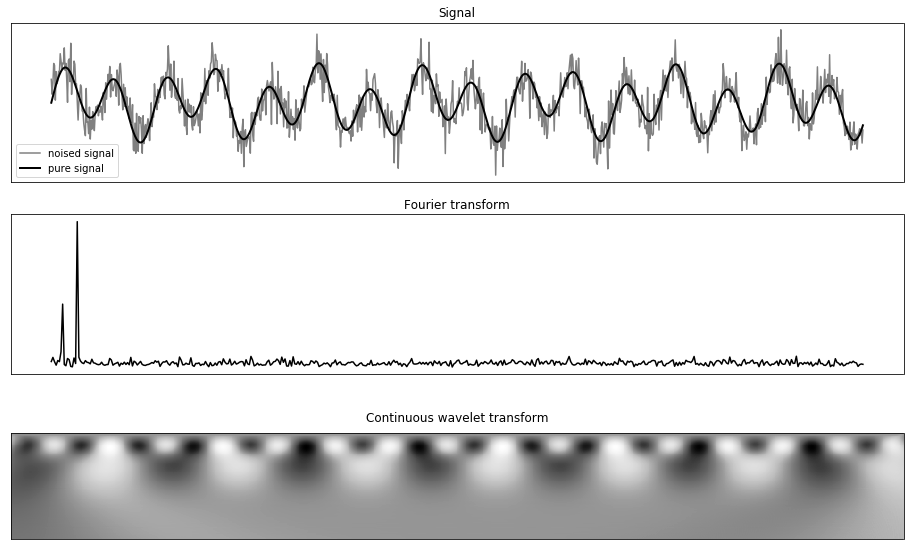
\includegraphics[scale=0.45]{./output_2_0.png}
	\end{center}
	\begin{center}
		Конкатенация двух синусоид:
		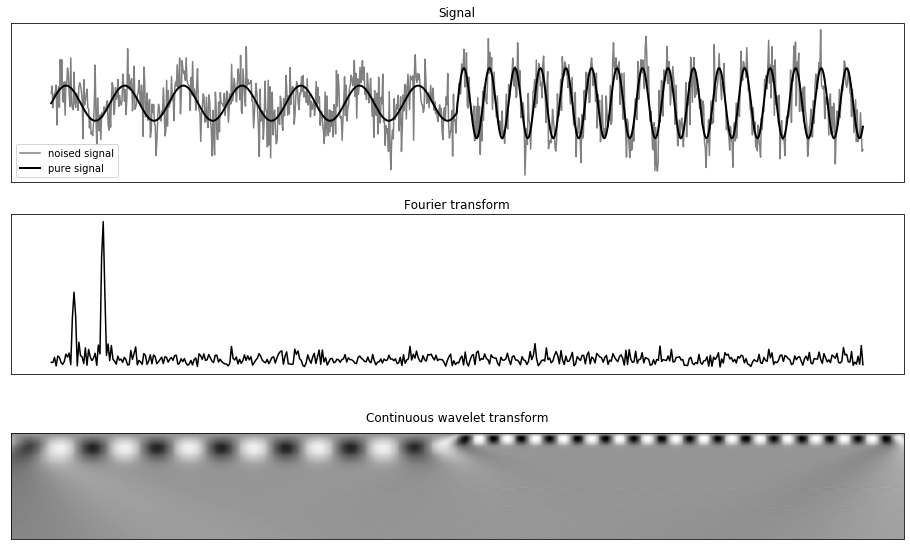
\includegraphics[scale=0.45]{./output_3_0.png}
	\end{center}

	Как мы можем увидеть, отличия в преобразовании Фурье вызваны только различными шумами и величиной пиков, различия же вейвлет коэффициентов видны даже визуально. Но все же существует оконное преобразование Фурье позволяющее частично избавиться от этого недостатка.
		
	\subsection{Сглаживание и сжатие временных рядов}
	
	При предсказывании временных рядов нам хочется искать закономерности, а не пытаться предсказать шум. Вейвлет преобразование позволяет сгладить данные и при этом уменьшить размерность.
	
	\begin{center}
		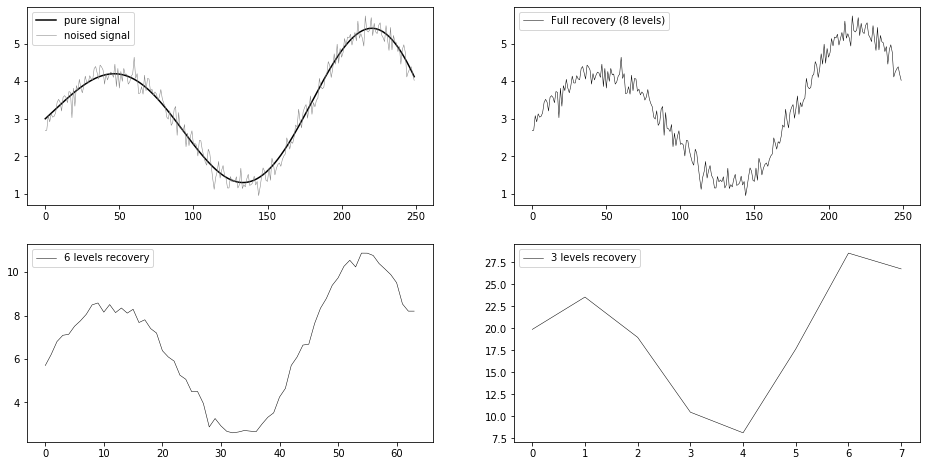
\includegraphics[scale=0.5]{./output_7_0.png}
	\end{center}

	Но снизить размер данных можно не только выбросив высокие частоты. Преобразование Хаара лучше поддается кодировке, что позволяет еще больше уменьшить размер.
	
	\subsection{Исследование стационарности временных рядов}
	
	Стационарность --- свойство процесса не менять свои характеристики со временем.
	
	\begin{itemize}
		\item Временной ряд справа не является стационарным, т.к. растет мат. ожидание, т.е. существует тренд.
		\begin{center}
			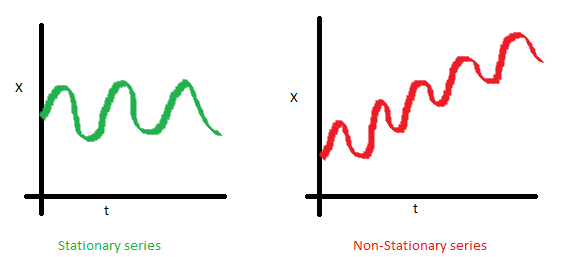
\includegraphics[scale=0.45]{./img1_1.png}
		\end{center}
		\item В этом случае у ряда растет дисперсия.
		\begin{center}
			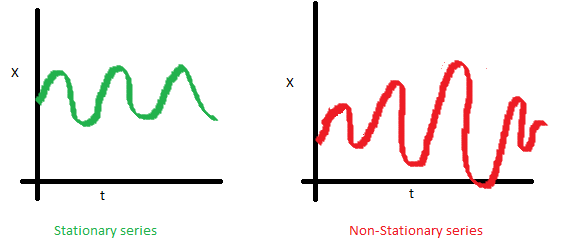
\includegraphics[scale=0.5]{./img1_2.png}
		\end{center}
		\item На последнем графике видно, что данные сжимаются друг к другу, т.е. есть непостоянство ковариаций.
		\begin{center}
			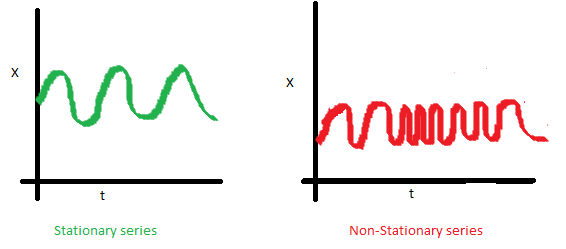
\includegraphics[scale=0.5]{./img1_3.png}
		\end{center}
	\end{itemize}
	
	Коэффициенты непрерывного преобразования можно использовать для определения стационарности. Для сравнения будем использовать статистический тест Дики-Фуллера.
	
	\begin{center}
		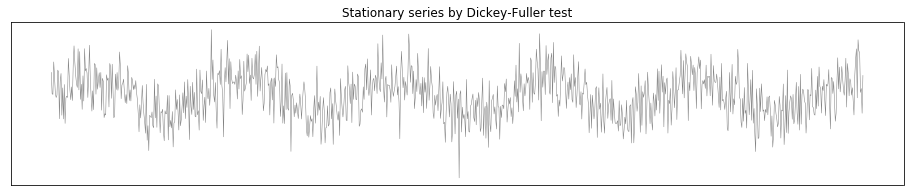
\includegraphics[scale=0.5]{./output_9_0.png}
		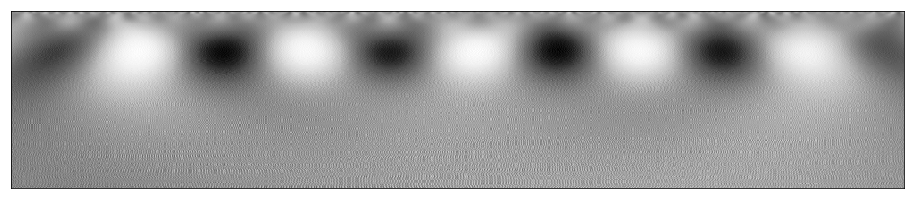
\includegraphics[scale=0.5]{./output_9_1.png}
		adf: -3.481848853184378 \\
		p-value: 0.008465675598229853 \\
		Critical values: {'1\%': -3.436, '5\%': -2.864, '10\%':
			-2.568}
	\end{center}

	Для данного ряда выражена периодичность, причем эта же периодичность прослеживается и в коэффициентах.
	
	\vspace{2em}
	
	\begin{center}
		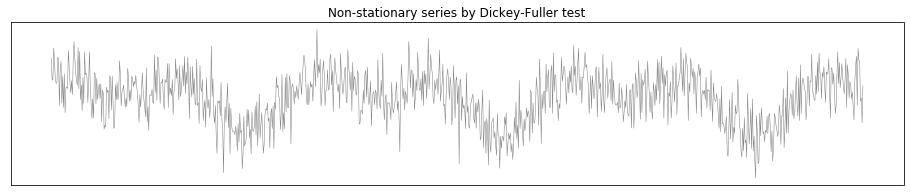
\includegraphics[scale=0.45]{./output_10_0.png}
		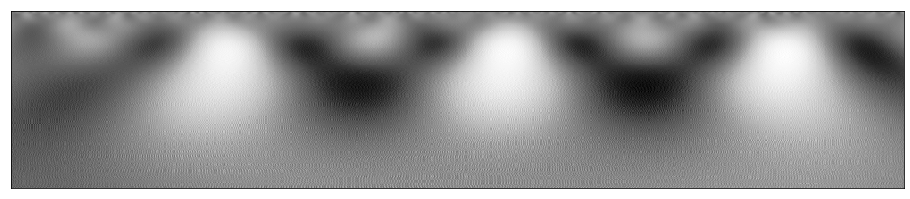
\includegraphics[scale=0.45]{./output_10_1.png}
		
		adf: -2.903023162949968 \\
		p-value: 0.0449975725101061 \\
		Critical values: {'1\%': -3.436, '5\%': -2.864, '10\%':
			-2.568}
	\end{center}

	Тут периодичность не так ярко выражена, но все еще хорошо видна в коэффициентах, при этом Тест говорит, что ряд не стационарен.
	
	\vspace{2em}
	
	\begin{center}
		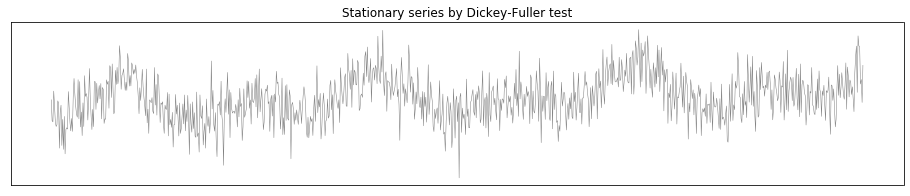
\includegraphics[scale=0.45]{./output_11_0.png}
		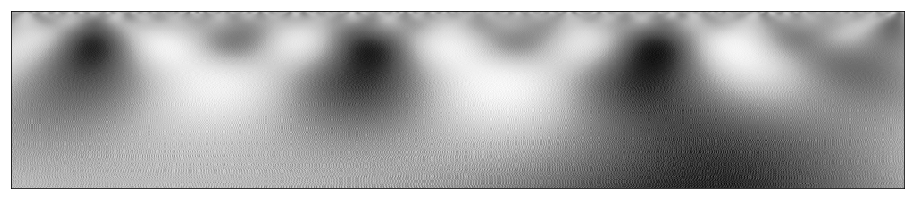
\includegraphics[scale=0.45]{./output_11_1.png}
		
		adf: -3.276199205944301 \\
		p-value: 0.015976475379125093 \\
		Critical values: {'1\%': -3.436, '5\%': -2.864, '10\%':
			-2.568}
	\end{center}
	
	Данный ряд выглядит вполне стационарным, о чем нам говорит и статистический тест, но на вейвлет-коэффициентах можно увидеть наличие тренда.
	
	\begin{center}
		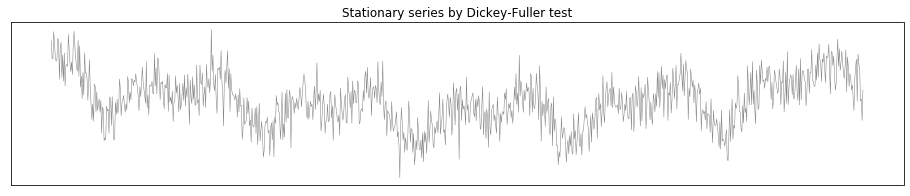
\includegraphics[scale=0.45]{./output_12_0.png}
		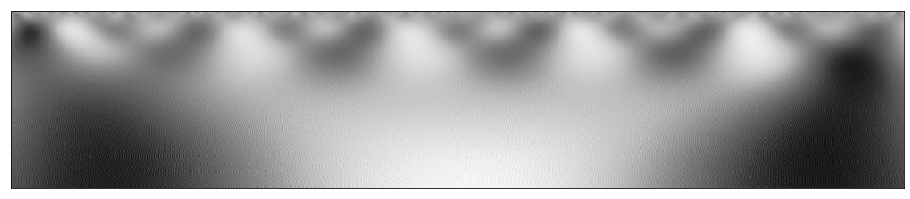
\includegraphics[scale=0.45]{./output_12_1.png}
		
		adf: -3.5973135357984862 \\
		p-value: 0.005812595366803051 \\
		Critical values: {'1\%': -3.436, '5\%': -2.864, '10\%':
			-2.568}
	\end{center}

	По этим коэффициентам можно определить наличие параболического тренда
	
	\vspace{2em}
	
	\begin{center}
		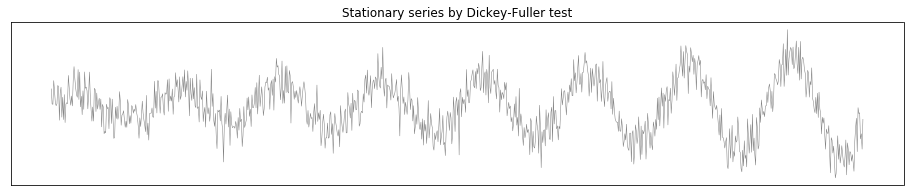
\includegraphics[scale=0.45]{./output_13_0.png}
		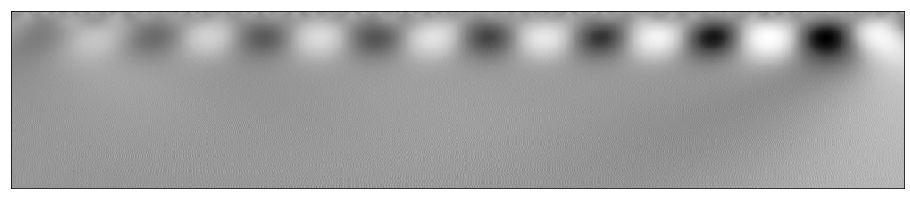
\includegraphics[scale=0.45]{./output_13_1.png}
		
		adf: -5.770885118947002 \\
		p-value: 5.39587787602044e-07 \\
		Critical values: {'1\%': -3.436, '5\%': -2.864, '10\%':
			-2.568}
	\end{center}
	
	Хоть тест говорит, что ряд стационарен, но мы наблюдаем увеличение дисперсии
	
	\subsection{Преимущества вейвлет-преобразования во временной \\ области}
	
	Проведем сравнение обычного статистического анализа на наборе данных о травматизме в 2015 году.
	
	После статистического анализа мы можем сказать, что:
	
	\begin{minipage}{0.45\textwidth}
		\begin{center}
			Всего было:
			\begin{itemize}
				\item В понедельник : 49868 случаев
				\item В вторник     : 46629 случаев
				\item В среду       : 46727 случаев
				\item В четверг     : 46798 случаев
				\item В пятницу     : 45269 случаев
				\item В субботу     : 49408 случаев
				\item В воскресенье : 50140 случаев
			\end{itemize}
		\end{center}
	\end{minipage}
	\hfill
	\begin{minipage}{0.45\textwidth}
		\begin{center}
			В среднем было:
			\begin{itemize}
				\item В понедельник : 959 случаев
				\item В вторник     : 897 случаев
				\item В среду       : 899 случаев
				\item В четверг     : 883 случаев
				\item В пятницу     : 871 случаев
				\item В субботу     : 950 случаев
				\item В воскресенье : 964 случаев
			\end{itemize}
		\end{center}
	\end{minipage}
	
	\vspace{2em}
	Проведем разложение на этих данных:
	\begin{center}
		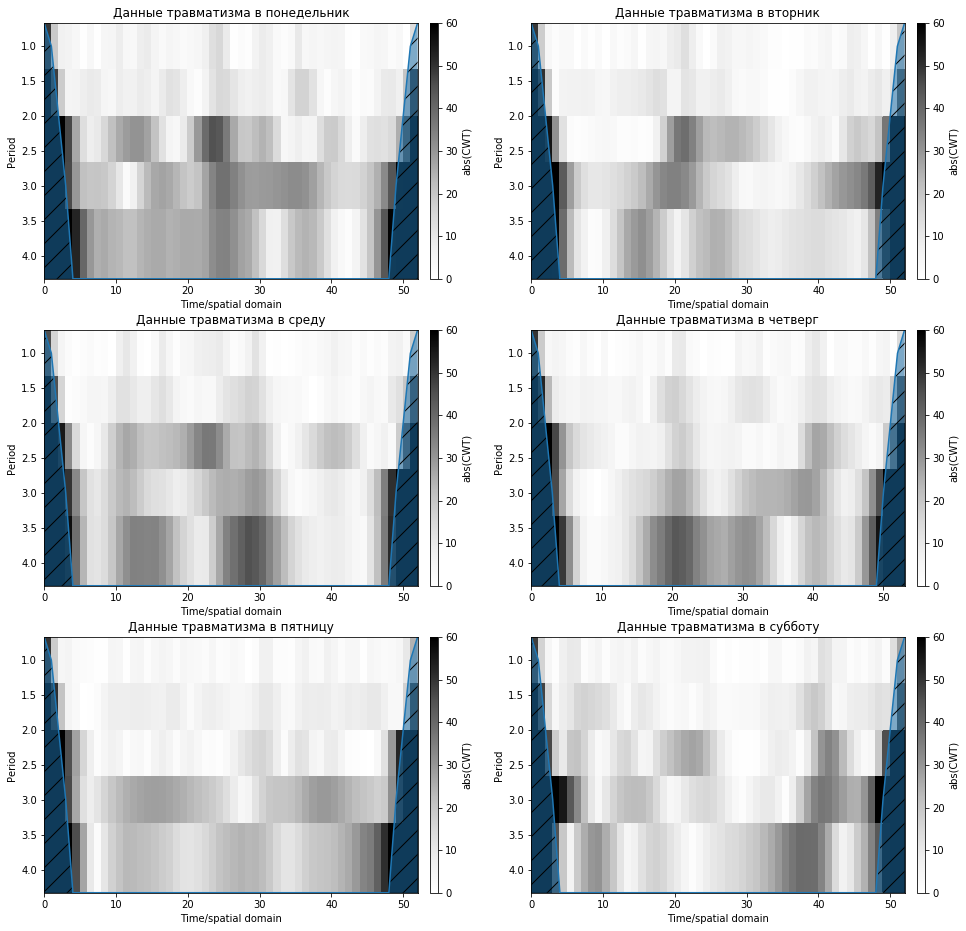
\includegraphics[scale=0.46]{./output_18_0.png}
		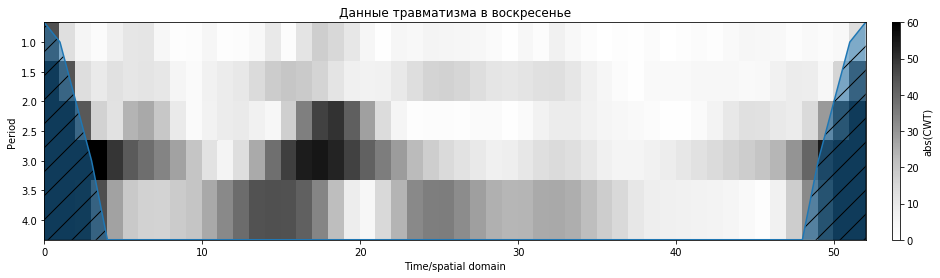
\includegraphics[scale=0.46]{./output_18_1.png}
	\end{center}
	
	Статистические данные позволяют узнать общую информацию.
	
	Черные пятна на спектрограмме соответствуют всплескам. По коэффициентам можно сказать, что, например, в воскресенье большинство случаев соответствуют апрелю-маю, а в четверг --- середине года. Также по данным мы можем увидеть, что внутри года закономерности не наблюдается. 
	
	\newpage
	
	\anonsection{Заключение}
	
	В курсовой работе получены следующие основные результаты:
	
	\begin{itemize}
		\item Изучены свойства вейвлетов, в частности вейвлетов Хаара
		\item Приведены математические основы для работы с вейвлетами
		\item Проведены компьютерные эксперименты по работе с дискретными и непрерывными вейвлетами, а в частности:
		\begin{itemize}
			\item Проведено сравнение с преобразованием Фурье
			\item Рассмотрено сглаживание и сжатие временных рядов
			\item Проведено исследование стационарности
		\end{itemize}
	\end{itemize}
	
	\newpage
	
	\begin{thebibliography}{8}
		\bibitem{Daubechies}
		I. Daubechies. Ten Lectures on Wavelets / I. Daubechies // Capital City Press, Montpelier, Vermont - 1992
		\bibitem{Vshivkov}
		F. Abramovich,. Wavelet analysis and its statistical applications / F. Abramovich,                      T. Bailey, and T. Sapatinas // JRSSD, (48):1–30 - 2000
		\bibitem{WaveletTransform}
		Wavelet transform --- Wikipedia [Электронный ресурс].  --- Режим доступа: https://en.wikipedia.org/wiki/Wavelet-transform, свободный.
		\bibitem{Haar}
		Haar wavelet – Wikipedia [Электронный ресурс]. – Режим доступа: https://en.wikipedia.org/wiki/Haar-wavelet, свободный.
		\bibitem{FourierTransform}
		Fourier transform --- Wikipedia [Электронный ресурс]. --- Режим доступа: https://en.wikipedia.org/wiki/Fourier-transform
		\bibitem{Morettin}
		Pedro A. Morettin. A wavelet analysis for time series / Pedro A. Morettin , Chang Chiann // Journal of Nonparametric Statistics - 2007
		\bibitem{Chui}
		Charles K. Chui. An Introduction to Wavelets / Charles K. Chui // Texas AM University, College Station, Texas - 2001
		\bibitem{TaoLi}
		Tao Li. A Survey on Wavelet Applications in Data Mining / Tao Li, Qi Li, Shenghuo Zhu, Mitsunori Ogihara // ACM SIGKDD Explorations Newsletter  - 2002
	\end{thebibliography}
	
	\newpage
	
	\anonsection{Приложение}
	
	\begin{lstlisting}[inputencoding={utf8}]

import pywt
import numpy as np
import pandas as pd
import statsmodels.api as sm
import matplotlib.pyplot as plt

import warnings
warnings.filterwarnings('ignore')

np.random.seed(0)
..............................
X_range = np.arange(1000)      

def describe(signal):
    plt.figure(figsize=(16, 10))
    signal_with_noise = signal + np.random.normal(0, 1, len(signal))

    plt.subplot(3, 1, 1)
    plt.plot(signal_with_noise, 'gray', label='noised signal')
    plt.plot(signal, 'black', label='pure signal', linewidth=2)
    plt.xticks(()), plt.yticks(())
    plt.title('Signal')
    plt.legend()

    plt.subplot(3, 1, 2)
    plt.plot(np.abs(np.fft.rfft(signal_with_noise)), 'black')
    plt.title('Fourier transform')
    plt.xticks(()), plt.yticks(())

    ax = plt.subplot(3, 1, 3)
    coef, freqs=pywt.cwt(signal ,np.arange(1, 120),'mexh')
    ax.matshow(coef, cmap='Greys')
    plt.title('Continuous wavelet transform')
    plt.xticks(()), plt.yticks(())
    plt.show()
..............................
describe(np.sin(X_range / 23) + 2 * np.sin(X_range / 10))
..............................
describe(np.append(np.sin(X_range[::2] / 23),
	       2 * np.sin(X_range[::2] / 10)))
..............................


from scipy import integrate

class wavelet_series:
    def __init__(self, g, levels=8):
        self.levels = levels
        mother_wavelet = lambda x: 0 if x < 0   else
                                   1 if x < 0.5 else
                                  -1 if x < 1   else 0

        self.scaling = lambda x: 1 if 0 <= x < 1 else 0

        self.basis = [[
            (lambda i, j: lambda x:
                2 ** (i / 2) * mother_wavelet(2**i * x - j))(i, j)
        for j in range(2 ** i)] for i in range(levels)]

        self.coef = [[
            integrate.quad(lambda x: g(x) * self.basis[i][j](x), 0, 1)[0] 
        for j in range(2 ** i)] for i in range(levels)]

        self.scaling_coef = integrate.quad(
            lambda x: g(x) * self.scaling(x), 0, 1)[0]

    def __call__(self, point):
        value = 0
        for i in range(self.levels):
            for j in range(2 ** i):
                value += self.coef[i][j] * self.basis[i][j](point)
        return value + self.scaling_coef * self.scaling(point)
..............................
g = lambda x: np.exp(x / 3) * np.sin(3 * x) + 3
xs = np.linspace(1e-8, 1 - 1e-8, 1000)

plt.figure(figsize=(16, 8))
for i in range(1, 7):
    f = wavelet_series(g, i)
    plt.subplot(2, 3, i)
    plt.plot(xs, list(map(g, xs)), 'grey', label='exp(x/3) sin(3x) + 3')
    plt.plot(xs, list(map(f, xs)), 'black',
             label='Wavelet-transform level %d' % i)
    plt.legend()

    if i == 5:
        plt.xlabel('Continues Haar transform')
plt.show()
..............................
def decomposition(signal, wavelet='Haar'):
    wavelet = pywt.Wavelet(wavelet)
    signal_with_noise = signal + np.random.normal(0, 0.2, len(signal))

    plt.figure(figsize=(16, 8))
    plt.subplot(2, 2, 1)
    plt.plot(signal, 'black', label='pure signal')
    plt.plot(signal_with_noise,'gray', 
             label='noised signal', linewidth=0.5)
    plt.legend()

    coefs = pywt.wavedec(signal_with_noise, wavelet, level=8)

    plt.subplot(2, 2, 2)
    plt.plot(pywt.waverec(coefs, wavelet), 'black',     
             label='Full recovery (8 levels)', linewidth=0.5)
    plt.legend()

    plt.subplot(2, 2, 3)
    plt.plot(pywt.waverec(coefs[:-2], wavelet), 'black', 
             label='6 levels recovery', linewidth=0.5)
    plt.legend()

    plt.subplot(2, 2, 4)
    plt.plot(pywt.waverec(coefs[:-5], wavelet), 'black', 
             label='3 levels recovery', linewidth=0.5)
    plt.legend()

    plt.show()
..............................
decomposition(g(np.linspace(0, 3, 250)))
..............................
def ShowSeries(series, wavelet='mexh'):
    test = sm.tsa.adfuller(series)

    plt.figure(figsize=(16, 3))
    plt.plot(series, 'Grey', linewidth=0.5)
    plt.xticks(())
    plt.yticks(())
    if test[0] > test[4]['5%']: 
        plt.title('Non-stationary series by Dickey-Fuller test')
    else:
        plt.title('Stationary series by Dickey-Fuller test')

    coef, freqs = pywt.cwt(series ,np.arange(1, 200), wavelet)
    plt.matshow(coef, cmap='Greys')
    plt.xticks(())
    plt.yticks(())
    plt.show()

print('adf: ', test[0])
print('p-value: ', test[1])
print('Critical values: ', test[4])
..............................
noise = np.random.normal(0, 1, 1000)
x_range = np.arange(1000)

ShowSeries(np.sin(x_range / 30) +
           noise)
..............................
ShowSeries(np.sin(x_range / 50) + 
           np.sin(x_range / 25 - 5) +
           noise)
..............................
ShowSeries(np.sin(x_range / 50) + 
           np.sin(x_range / 25 - 2) +
           x_range / 500 + 
           noise * 1.3)
..............................
ShowSeries(np.sin(x_range / 30 + 2) + 
           np.sin(x_range / 15) + 
           ((x_range - len(x_range) / 2) / 300)**2 +
           noise)
..............................
ShowSeries((np.sin(x_range / 20)) * (x_range + len(x_range))**2 +
           noise * 1e6)
..............................
df = pd.read_csv('nss15.csv')

time = pd.to_datetime(df.treatmentDate, format='%m/%d/%Y')
timeseries = pd.Series(np.ones(len(time)), index=sorted(time),
                       dtype=np.int64)
                  .resample('D').sum()
..............................
from scaleogram import cws

timeseries.index = pd.Series(timeseries.index)
                       .apply(lambda day: day.weekday())

dayweeks = ['понедельник', 'вторник', 'среду', 'четверг',
            'пятницу', 'субботу', 'воскресенье']

for i in range(7):
    print('В {:12s}: {} случаев'.format(
              dayweeks[i], timeseries[i].sum()))

for i in range(7):
    print('В {:12s}: {} случаев'.format(
              dayweeks[i], round(timeseries[i].mean())))
..............................
plt.figure(figsize=(16, 16), dpi=600)

for i in range(6):
    ax = plt.subplot(3, 2, i + 1)
    cws(timeseries[i], cmap='Greys', ax=ax, clim=[0, 60],
        title='Данные травматизма в %s' % dayweeks[i])
    plt.show()

plt.figure(figsize=(16, 4))
ax = plt.subplot(1, 1, 1)
cws(timeseries[6], cmap='Greys', ax=ax, clim=[0, 60], 
    title='Данные травматизма в %s' % dayweeks[i])
plt.show()

	\end{lstlisting}
	
	\newpage
	
	
\end{document}